%%%%%%%%%%%%%%%%%%%%%%%%%%%%%%%%%
%
%       EXERCÍCIO
%
%%%%%%%%%%%%%%%%%%%%%%%%%%%%%%%%%

\ifdefstring{\atividade}{prova}{%
    \ifdefstring{\modo}{objetivo}{%
        \renewcommand{\valorquestao}{\ValorQObj\ ponto}
    }{%
        \renewcommand{\valorquestao}{\ValorQDisc\ pontos}
    }%
}%

\begin{exercicioBanco}[\valorquestao]
Na figura estão representadas, em um plano cartesiano, duas circunferências: \(C_{1}\) (de raio 3 e centro \(O_{1}\)) e  \(C_{2}\) (de raio 1 e centro \(O_{2}\)), tangentes entre si, e uma reta \(t\) tangente às duas circunferências nos pontos \(P\) e \(Q\).

\begin{center}
    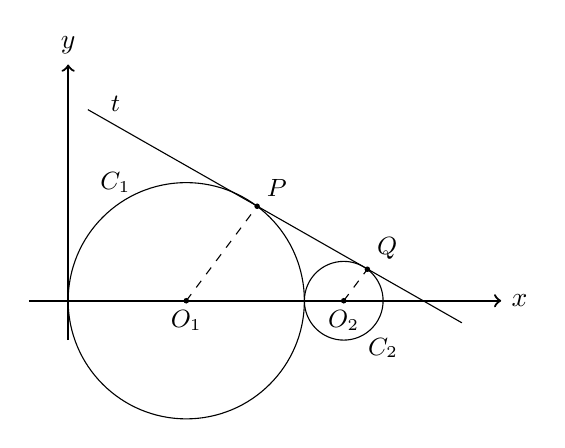
\begin{tikzpicture}[scale=0.5]
        % Eixos
        \draw[->,thick] (-1,0) -- (11,0) node[right] {$x$};
        \draw[->,thick] (0,-1) -- (0,6) node[above] {$y$};

        % Centros
        \coordinate (O1) at (3,0);
        \coordinate (O2) at (7,0);

        % Raios
        \def\rA{3}
        \def\rB{1}

        % Círculos
        \draw (O1) circle (\rA);
        \draw (O2) circle (\rB);

        % Pontos dos centros
        \fill (O1) circle (2pt) node[below] {\small$O_1$};
        \fill (O2) circle (2pt) node[below] {\small$O_2$};

        % Pontos de tangência (aproximados manualmente)
        \draw[domain=0.5:10, smooth, variable=\x]
            plot ({\x}, {-0.57*\x + 5.14});
        
        \node at (1.2,5) {\small$t$};
        
        \coordinate (P) at (4.8,2.4);
        \coordinate (Q) at (7.6,0.8);

        \fill (P) circle (2pt) node[above right] {\small$P$};
        \fill (Q) circle (2pt) node[above right] {\small$Q$};

        % Segmentos pontilhados (raios até a tangente)
        \draw[dashed] (O1) -- (P);
        \draw[dashed] (O2) -- (Q);

        % Rótulos dos círculos
        \node at (1.2,3) {\small$C_1$};
        \node at (8,-1.2) {\small$C_2$};
    \end{tikzpicture}
\end{center}

Nessas condições, determine a equação da reta t.

% Define as alternativas
\newcommand{\alternativas}{%
    \begin{center}
        \begin{tabularx}{\textwidth}{XXX}
            (a) \(y = -\sqrt{3}x + 3\sqrt{3}\). &
            (b) \(y = -\dfrac{\sqrt{3}}{3}x + 3\sqrt{3}\). &
            (c) \(y = -x + 4\). \\[15pt]
            (d) \(y = -\dfrac{2}{3}x + 4\). &
            (e) \(y = -\dfrac{4}{5}x + 4\).
        \end{tabularx}
    \end{center}
}

% Define a resposta correta
\newcommand{\resposta}{B}

% Lógica condicional para exibição
\ifdefstring{\atividade}{lista}{%
    \alternativas
    \vspace{0.5em}
    
    \noindent\textbf{Resposta:} letra \textbf{\resposta}.
}{%
    \ifdefstring{\modo}{objetivo}{%
        \alternativas
    }{%
        % modo = discursiva → não mostra alternativas
    }
}
\end{exercicioBanco}

